\medskip

\textbf{Partie A :}

\medskip

\begin{enumerate}
	\item $\bullet~$Limite en 0:

$\lim\limits_{x\to 0} x^2 =0$ et, d'après la propriété des croissances comparées : \quad $\lim\limits_{x\to 0}x\ln(x)=0$

Par limite de la somme,  on a donc :\quad $\lim\limits_{x\to 0} x^2-x\ln(x)=0$

$\bullet~$Limite en $+\infty$:

$f(x)=x^2-x\ln(x)=x^2 \left(1-\dfrac{\ln(x)}{x}\right)$

	Par croissances comparées $\lim\limits_{x\to +\infty}\dfrac{\ln(x)}{x}=0$ donc, par limite de la somme, $\lim\limits_{x\to +\infty}\left( 1- \dfrac{\ln(x)}{x}\right)=1$

	De plus $\lim\limits_{x\to +\infty} x^2 =+\infty$, donc, par limite du produit,  $\lim\limits_{x\to +\infty } x^2 \left(1-\dfrac{\ln(x)}{x}\right)=+\infty$

	\item  Pour tout réel $x$ strictement positif, on a: $f'(x) =2x -1 \times \ln(x) -x \times \dfrac{1}{x}= 2x -1 -\ln(x)$.

	\item  Pour tout réel $x$ strictement positif, on a: $f''(x) =2- 0 - \dfrac{1}{x}= \dfrac{2x}{x} -\dfrac{1}{x}= \dfrac{2x-1}{x}$.

	\item  	Déterminons le signe de $2x-1$ :

	$\begin{aligned}[t] 2x-1 >0 &\iff 2x > 1 \\
	&\iff x>\dfrac{1}{2}\end{aligned}$

	L'image pertinente est : (les limites aux bornes ne sont pas attendues)


	$f'\left( \dfrac{1}{2}\right)= 2 \times \dfrac{1}{2}-1-\ln\left(\dfrac{1}{2} \right)= 1-1+\ln(2)=\ln(2)$

	On a donc :

	\begin{tikzpicture}
		\tkzTabInit[lgt=3,espcl=4]{$x$/1,signe de $2x-1$/0.6,signe de $x$/0.6,signe de $f''(x)$/0.8,variations de $f'$/2}{0,{$\dfrac{1}{2}$},$+\infty$}
		\tkzTabLine{t,-,z,+,}
		\tkzTabLine{z,+,t,+,}
		\tkzTabLine{d,-,z,+,}
		\tkzTabVar{D+/,-/$\ln(2)$,+/}
	\end{tikzpicture}

	\item Le minimum  de la fonction $f'$ sur $]0~;~+\infty[$  est donc $\ln(2)$ qui est strictement positif,  donc, sur $]0~;~+\infty[$, $f'(x)>0$ et donc, la fonction $f$ est strictement croissante sur   $]0~;~+\infty[$.
\end{enumerate}


\textbf{Partie B :}

\medskip

\begin{enumerate}
	\item Pour tout réel $x$ strictement positif, on a: $g'(x) =1 - \dfrac{1}{x}= \dfrac{x-1}{x}$.

Déterminons le signe de $x-1$ :

$ x-1 >0 \iff x > 1 $

L'image pertinente est : (les limites aux bornes ne sont pas attendues)

$g(1)= 1-\ln(1)=1-0=1$

On a donc :
	\begin{tikzpicture}
		\tkzTabInit[lgt=3,espcl=4]{$x$/0.6,signe de $x-1$/0.6,signe de $x$/0.6,signe de $g'(x)$/0.8,variations de $g$/2}{0,1,$+\infty$}
		\tkzTabLine{,-,z,+,}
		\tkzTabLine{z,+,t,+,}
		\tkzTabLine{d,-,z,+,}
		\tkzTabVar{D+/,-/1,+/}
	\end{tikzpicture}

	\item $\begin{aligned}[t] f(x) = x &\iff x = x^2-x\ln(x) \\
	&\iff 0 = x^2-x-x\ln(x) \\
	&\iff 0 = x\left( x-1-\ln(x)\right)\\
	&\iff 0 = x-1-\ln(x) \quad \text{car } x>0 \quad \text{ donc } x\neq0 \\
	& \iff 1 = x-\ln(x)\\
	&\iff 1 = g(x)\\
	&\iff x = 1 \end{aligned}$

L'équation $f(x)=x$ admet une unique solution sur $]0~;~+\infty[$, cette solution est $x=1$.
\end{enumerate}

\medskip

\textbf{Partie C :}

\medskip

\begin{enumerate}
	\item Montrons par récurrence que pour tout entier naturel  $n$, \quad$\dfrac{1}{2} \leqslant u_n \leqslant u_{n+1} \leqslant 1$.



\emph{Initialisation :} Calculons $u_1$. $u_1 = f(u_0) = f\left(\dfrac{1}{2} \right) = \left(\dfrac{1}{2}\right)^2-\dfrac{1}{2}\ln \left(\dfrac{1}{2}\right)= \dfrac{1}{4} +\dfrac{\ln(2)}{2}\approx 0,597 $.

On constate que l'inégalité est vraie pour $n = 0$, on a bien : \quad $ \dfrac{1}{2}\leqslant u_0 \leqslant u_1 \leqslant 1$.

\smallskip

\emph{Hérédité :} Soit $n \in \N$, tel que \quad $ \dfrac{1}{2}\leqslant u_n \leqslant u_{n+1} \leqslant 1$.

Montrons que l'inégalité est vraie au rang suivant :

Par hypothèse de récurrence on a :

$ \begin{aligned}[t] \dfrac{1}{2}\leqslant u_n \leqslant u_{n+1} \leqslant 1
&\implies f\left(\dfrac{1}{2}\right)\leqslant f(u_n) \leqslant f(u_{n+1}) \leqslant f(1)\\
&\hphantom{\implies}\quad \text{car $f$ est strictement croissante sur }]0~;~+\infty[\\
&\implies f\left(\dfrac{1}{2}\right)\ \leqslant u_{n+1 } \leqslant u_{n+2} \leqslant 1\\
&\hphantom{\implies}\quad \text{car $f$ est la fonction de récurrence de la suite } (u_n)\\
&\implies \dfrac{1}{2} \leqslant u_{n+1 } \leqslant u_{n+2} \leqslant 1\\
&\hphantom{\implies}\quad \text{car } f\left(\dfrac{1}{2}\right)\ \approx 0,60 >\dfrac{1}{2} \\\end{aligned}$

Ceci montre que les  inégalités sont vraies au rang $n + 1$.

\smallskip

\emph{Conclusion :} Les inégalités sont vraies au rang 0, et si elle sont vraies au rang $n$ naturel, elles sont vraies au rang suivant $n + 1$, donc, en vertu du principe de récurrence, on a :

$\forall n \in \N,\quad \dfrac{1}{2} \leqslant u_{n} \leqslant u_{n+1} \leqslant 1$.

	\item On a notamment :
		\begin{itemize}
			\item $\forall n \in \N,\quad u_{n} \leqslant u_{n+1}$. \quad La suite $(u_n)$ est donc  croissante.
			\item $\forall n \in \N,\quad \dfrac{1}{2} \leqslant u_{n}\leqslant 1$. \quad La suite $\left(u_n\right)$ est donc bornée par $\dfrac{1}{2}$ et 1.
		\end{itemize}

La suite étant croissante et majorée, on en déduit qu'elle est convergente, vers une limite $\ell$ vérifiant $\dfrac{1}{2} \leqslant \ell \leqslant 1$
		\item  La suite $\left(u_n\right)$ est une suite convergente, définie par récurrence par la relation $u_{n+1} = f\left(u_n\right)$, où la fonction $f$ est continue (car dérivable) sur $]0~;~+\infty[$, intervalle qui contient la limite $\ell$ de la suite.

D'après le théorème \og du point fixe \fg{}, on en déduit que la limite ne peut être qu'une solution de l'équation $f(x) = x$ dans l'intervalle  $]0~;~+\infty[$.

D'après la question \textbf{2.} de la \textbf{Partie B}, cette équation n'a qu'une solution dans  l'intervalle $]0~;~+\infty[$ :  1.

La suite $\left(u_n\right)$ converge donc vers $\ell = 1$.
\end{enumerate}

\bigskip
